\begin{center}4.\end{center}
\noindent\hspace*{\parindent}Um dies durch ein einfaches Beispiel zu erläutern, seien \(A,a,a',A'\) reelle Grössen, jede folgende algebraisch grösser als die vorhergehende, d. i. \(a-A\), \(a'-a\), \(A'-a'\) alle positiv; und auf ähnliche Weise verhalten sich die reellen Grössen \(B,b,b',B'\). Ich bezeichne die acht complexen Grössen
\[
\begin{gathered}
A+Bi,\quad A'+Bi,\quad A+B'i,\quad A'+B'i,\\
a+bi,\quad a'+bi,\quad a+b'i,\quad a'+b'i
\end{gathered}
\]
\noindent der Reihe nach mit \(C^{0,0},\,C^{1,0},\,C^{0,1},\,C^{1,1},\,c^{0,0},\,c^{1,0},\,c^{0,1},\,c^{1,1}\). Ferner die Schicht complexer Grössen \(x+yi\), wo \(x\) zwischen \(A\) und \(A'\), hingegen \(y\) zwischen \(B\) und \(B'\) liegt, mit \(S\). Eben so diejenige Schicht, wo \(x\) zwischen \(a\) und \(a'\), hingegen \(y\) zwischen \(b\) und \(b'\) liegt, mit \(s\). Endlich bemerke man, dass \(S\) begrenzt wird durch den geschlossenen Zug \(Z\), zusammengesetzt aus vier partiellen Zügen von \(C^{00}\) nach \(C^{10}\), von \(C^{10}\) nach \(C^{11}\), von \(C^{11}\) nach \(C^{01}\) und von \(C^{01}\) nach \(C^{00}\), und zwar so, dass im ersten und dritten Stück der imaginäre Theil constant bleibt, im zweiten und vierten hingegen der reelle. Auf ähnliche Weise sei \(z\) der geschlossene Zug, welcher die Schicht \(s\) begrenzt, und dessen vier Bestandtheile man hat, wenn man in denen von \(Z\) nur überall \(C\) gegen \(c\) vertauscht. Man erkennt leicht, dass auf diese Weise sowohl die Schicht \(S\)
\clearpage\SourceLeaf{418}\ArithmeticHead{411}{R}{CONVERGENZ DER ENTWICKLUNG PERIODISCHER FUNCTIONEN.}
\noindent zu dem Zuge \(Z\), als die Schicht \(s\) zu dem Zuge \(z\), wenn in den beiden Zügen die angegebene Folgeordnung vorausgesetzt wird, ein positives Verhältniss haben, oder dass diese Folgeordnungen für \(Z\) in Beziehung auf \(S\) und für \(z\) in Beziehung auf \(s\) gleiche sind.

Sondern wir nun aber aus den complexen Grössen \(S\) diejenigen aus, welche die Schicht \(s\) und zugleich diejenigen, welche den Zug \(z\) bilden, so bleibt Eine zusammenhängende Schicht übrig, die ich mit \(\Sigma\) bezeichne, und von welcher die zwei Züge \(Z,z\) die vollständige Begrenzung bilden. In Beziehung auf diese Schicht \(\Sigma\) sind nun die obigen Folgeordnungen in den Zügen nicht gleiche sondern entgegengesetzte: der Folgeordnung \(C^{00}\ C^{10}\ C^{11}\ C^{01}\ C^{00}\) gleich würde diese sein: \(c^{00}\ c^{01}\ c^{11}\ c^{10}\ c^{00}\). Man vergl. die räumliche Darstellung, wo durch die Pfeile die gleichen Folgeordnungen angedeutet sind.
\begin{center}
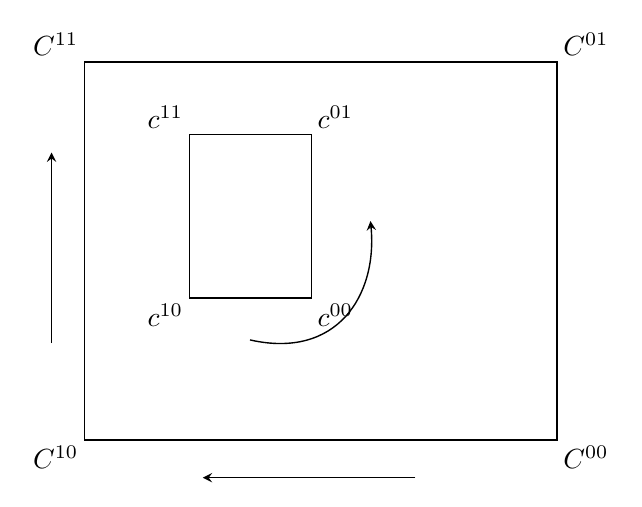
\begin{tikzpicture}[x=1cm,y=1cm,line width=.5pt]
\draw (0,0) rectangle (6,4.8);
\draw (1.33,1.8) rectangle (2.88,3.88);
\node[above left,inner sep=2pt] at (0,4.8) {\(C^{11}\)};
\node[above right,inner sep=2pt] at (6,4.8) {\(C^{01}\)};
\node[below left,inner sep=2pt] at (0,0) {\(C^{10}\)};
\node[below right,inner sep=2pt] at (6,0) {\(C^{00}\)};
\node[above left,inner sep=2pt] at (1.33,3.88) {\(c^{11}\)};
\node[above right,inner sep=2pt] at (2.88,3.88) {\(c^{01}\)};
\node[below left,inner sep=2pt] at (1.33,1.8) {\(c^{10}\)};
\node[below right,inner sep=2pt] at (2.88,1.8) {\(c^{00}\)};
\draw[->,>=stealth] (-.42,1.23)--(-.42,3.65);
\draw[->,>=stealth] (4.2,-.48)--(1.5,-.48);
\draw[->,>=stealth] (2.1,1.27) .. controls (3.2,1.02) and (3.72,1.83) .. (3.63,2.78);
\end{tikzpicture}
\end{center}
\begin{center}5.\end{center}
\noindent\hspace*{\parindent}Es muss hier noch hervorgehoben werden der Satz, dass eine Schicht \(\Sigma\), die durch zwei oder mehrere geschlossene Züge begrenzt ist, sich in eben so viele partielle Schichten zerlegen lässt, die jede nur von Einem Zuge begrenz\raisebox{.45ex}{t} werden. Es wird zum Beweise dieses Satzes nur nöthig sein, zu zeigen, dass allemahl \(\Sigma\) sich in zwei andere Schichten \(\Sigma'\) und \(\Sigma''\) zerlegen lasse, so dass \(\Sigma'\) nur durch Einen Zug begrenzt werde, und die Anzahl der Züge, durch welche \(\Sigma''\) begrenzt ist, um eine Einheit kleiner sei, als die Zahl der Grenzzüge von \(\Sigma\). Es seien \(Z\) und \(z\) zwei geschiedene Grenzzüge von \(\Sigma\), \(\zeta=Cc\), \(\zeta'=C'c'\) zwei andere Züge, so beschaffen, dass ihre Anfänge \(C\) und \(C'\) zu \(Z\), und die Enden \(c\) und \(c'\) zu \(z\) gehören, dass sie selbst keine Stelle gemein haben, und dass die Schicht, welche durch den geschlossenen Zug \(CC'c'cC\) begrenzt wird (wo \(CC',\,cc'\) beziehungsweise Theile von \(Z,z\) sind) ganz der Schicht \(\Sigma\) angehört, also einen Theil derselben ausmacht. Von der Möglich-
\par\vfill\hfill{\small 52\textsuperscript{*}}\par
\clearpage\SourceLeaf{419}\ArithmeticHead{412}{L}{ANALYSIS. NACHLASS.}
\noindent keit, diesen Bedingungen Genüge zu leisten, überzeugt man sich leicht, indem man erwägt, dass, in Folge des stetigen Zusammenhangs der Schicht \(\Sigma\), die zwei Züge \(Z,z\) sich durch einen ganz dieser Schicht angehörenden Zug \(Cc\) verbinden lassen, und dass man nöthigenfalls den zweiten Zug \(C'c'\) dem ersten so nahe wie man will nehmen darf. Wir haben also in der durch den Zug \(CC'c'cC\) begrenzten Schicht das geforderte \(\Sigma'\); nennt man das, was nach Absonderung derselben von \(\Sigma\) übrig bleibt, \(\Sigma''\), so werden dazu als Begrenzung gehören: erstlich diejenigen Züge, welche etwa noch ausser \(Z\) und \(z\) die Begrenzung von \(\Sigma\) bildeten, zweitens anstatt dieser beiden Züge \(Z,z\) der einfache gleichfalls geschlossene Zug \(Ccc''c'C'C''C\), wo \(c''\) eine beliebige Stelle in dem nicht geschlossenen Zuge bedeutet, welcher von \(z\) übrig bleibt, wenn man \(cc'\) davon absondert, und eben so \(C''\) eine beliebige Stelle von \(Z\) ausserhalb \(CC'\).

Es liesse sich übrigen[s] auch nachweisen, dass auf diese Weise \(\Sigma''\) wirklich Eine nach der Stetigkeit zusammenhängende Schicht bildet, was ich aber hier unterlasse, theils weil dazu noch einige anderweitige Erörterungen erforderlich sein würden, theils weil für gegenwärtigen Zweck zureicht, dass \(\Sigma''\), möge es Eine einzige zusammenhängende [Schicht] oder mehrere getrennte vorstellen, gewiss zusammen eine um eine Einheit geringere Anzahl von geschlossenen Grenzzügen darbietet als \(\Sigma\).

Man bemerke noch, dass in der Gesammtheit der Grenzzüge von \(\Sigma'\) und \(\Sigma''\) wieder erscheinen: erstlich die Grenzzüge von \(\Sigma\), und dann noch dazu die Züge \(\zeta\) und \(\zeta'\), und zwar jeder zweimal. Man sieht aber leicht, dass in \(\zeta\) als Grenzzug von \(\Sigma'\), und in \(\zeta\) als Grenzzug von \(\Sigma''\) entgegengesetzte Folgeordnungen gelten müssen, wenn diese Schichten gleiches Verhältniss dazu haben sollen, und dasselbe gilt von \(\zeta'\). In denjenigen Anwendungen also, in welchen zwei an sich gleiche aber in entgegengesetzten Folgeordnungen vorkommende Züge wie einander destruirend betrachtet werden können, kann man die Totalität der Grenzzüge von \(\Sigma\) der Totalität der Grenzzüge von \(\Sigma'\) und \(\Sigma''\) gleich setzen, und demnach auch der Totalität der einfachen Grenzzüge sämmtlicher aus weiterer Zerlegung hervorgehender Schichten.
